\documentclass[11pt,a4paper]{article}
\usepackage[utf8]{inputenc}
\usepackage[T1]{fontenc}
\usepackage{lmodern}
\usepackage[margin=1in]{geometry}
\usepackage{amsmath,amssymb,bm}
\usepackage{graphicx}
\usepackage{booktabs}
\usepackage{tabularx}
\usepackage{array}
\usepackage{longtable}
\usepackage{enumitem}
\usepackage{xcolor}
\usepackage{framed}
\usepackage{caption}
\usepackage{titlesec}
\usepackage{tikz}
\usetikzlibrary{arrows.meta,positioning,shapes.geometric,fit,backgrounds}
\usepackage[round,authoryear]{natbib}
\usepackage[hidelinks]{hyperref}
\usepackage{microtype}

\definecolor{shadecolor}{gray}{0.94}
\definecolor{accent}{HTML}{1F4E79}
\titleformat{\section}{\normalfont\large\bfseries\color{accent}}{\thesection}{0.6em}{}
\titleformat{\subsection}{\normalfont\bfseries}{\thesubsection}{0.5em}{}
\newcolumntype{Y}{>{\raggedright\arraybackslash}X}
\captionsetup{font=small,labelfont=bf}
\setlist{nosep,leftmargin=1.4em}

\newcommand{\NTrain}{31,656}
\newcommand{\NTest}{13,566}
\newcommand{\NFeat}{103}
\newcommand{\PosRate}{24.8\%}
\newcommand{\BestAcc}{0.848}
\newcommand{\BestModel}{Logistic Regression}
\newcommand{\RFMIA}{0.592}
\newcommand{\RFAdv}{0.108}
\newcommand{\AIacc}{0.838}
\newcommand{\AIbase}{0.677}
\newcommand{\AIleak}{0.161}
\newcommand{\FracUnique}{13.8\%}
\newcommand{\PADCAincome}{0.840}
\newcommand{\PADCAsex}{0.689}
\newcommand{\PCAsex}{1.000}


\begin{document}

% ------------------------------------------------------------------ cover
\begin{titlepage}
\centering
\vspace*{1.2cm}
{\large Security and Privacy for Machine Learning (Honors)}\\[0.3cm]
{\large\bfseries Internal Assessment 1}\\[0.2cm]
{\normalsize Problem Formulation and Preliminary Implementation}\\[1.6cm]
\rule{\textwidth}{0.4pt}\\[0.5cm]
{\LARGE\bfseries Which Privacy Layer Stops Which Attack?}\\[0.4cm]
{\large An Attack-Grounded Comparison of Central DP, Local DP,\\
Anonymisation and Compressive Privacy for Census-Income Prediction}\\[0.5cm]
\rule{\textwidth}{0.4pt}\\[2.2cm]
\begin{tabular}{rl}
\textbf{Name} & Deon Ajit Menezes\\[4pt]
\textbf{Roll No.} & 16014223030\\[4pt]
\textbf{Batch} & B1\\[4pt]
\textbf{Assessment} & IA-1 (20 marks)\\
\end{tabular}
\vfill
{\small Submitted as an individual integrated research work spanning all five course modules.}
\end{titlepage}

\tableofcontents
\vspace{0.6cm}

% ------------------------------------------------------------------ rubric map
\begin{shaded}
\noindent\textbf{Rubric-compliance map.} This report is organised to mirror the five IA-1
criteria; the table below points each required evidence item to where it appears.
\end{shaded}
\begin{center}\small
\begin{tabularx}{\textwidth}{>{\bfseries}p{3.2cm}Yc}
\toprule
IA-1 criterion & Evidence in this report & Section\\
\midrule
Problem \& module mapping & Problem statement, objectives, scope, five-module mapping table & \S\ref{sec:problem}\\
Conceptual understanding & Concept note, workflow diagram, implement/demonstrate/analyse split & \S\ref{sec:concept}\\
Dataset preparation & Provenance table, cleaning log, hashes & \S\ref{sec:data}\\
Initial implementation & Baselines, attack suite, one mechanism per module, code & \S\ref{sec:impl}\\
Preliminary evaluation & Observations, limitations, evaluation plan, contribution statement & \S\ref{sec:eval}\\
\bottomrule
\end{tabularx}
\end{center}

% ================================================================== 1
\section{Problem Definition and Module Mapping}\label{sec:problem}

\subsection{Problem statement}
An organisation trains a binary classifier that predicts whether an individual's
income exceeds \$50K from personal census records. The same record is exposed at
\emph{four distinct points} in the machine-learning pipeline, and each exposure
invites a different privacy attack with a different natural defence:
\begin{enumerate}
\item \textbf{Collection} from individuals by an untrusted curator $\Rightarrow$ attribute disclosure.
\item \textbf{Publishing} a record-level table to analysts $\Rightarrow$ linkage re-identification and homogeneity attacks.
\item \textbf{Sharing} features with a third-party ML service $\Rightarrow$ sensitive-attribute inference.
\item \textbf{Deploying} the trained model as a query API $\Rightarrow$ membership inference.
\end{enumerate}
The course offers a different privacy technology for each layer: local differential
privacy (Module~3), $k$-anonymity and its refinements (Module~4), compressive
privacy (Module~5), and central differential privacy (Module~2); Module~1 supplies
the threat models used to \emph{measure} them.

\subsection{Significance, scope and objectives}
In the privacy-preserving ML literature each of these defences is almost always
evaluated in isolation, on a different dataset and against a different yardstick,
which makes it impossible to answer the practitioner's real question: \emph{given a
specific exposure and a specific attack, which mechanism should I deploy, and what
does it cost?} The contribution of this work is to place all four defence families
on \textbf{one dataset, one utility metric and one attack suite}, and to summarise
the outcome as a \emph{defence-coverage matrix}.

\noindent\textbf{Objectives.} (O1) Build an income classifier and a reusable attack
suite (membership inference, attribute inference, linkage). (O2) Implement one
representative mechanism from every module. (O3) Measure each mechanism's
privacy gain and utility cost on common axes. (O4) In IA-2, assemble the
coverage matrix and test a layered combination.

\noindent\textbf{Scope.} The study is empirical and single-dataset (UCI Adult, with an
IA-2 replication on ACSIncome). Cryptographic approaches (homomorphic encryption,
secure multiparty computation, federated learning) are treated analytically, not
implemented, because they protect \emph{computation} rather than alter the
privacy--utility trade-off this study measures.

\noindent\textbf{Expected outcome.} A reproducible benchmark and a coverage matrix
stating, per attack, which mechanism neutralises it and the accuracy sacrificed.

\subsection{Mapping to all five modules}
Table~\ref{tab:modmap} maps every module (and the sub-units that are exercised) to
its role in the project. The treatment code is
\textbf{I}=implemented, \textbf{E}=experimentally evaluated,
\textbf{D}=demonstrated, \textbf{A}=analytically discussed.

\begin{longtable}{>{\bfseries}p{1.5cm}p{6.8cm}p{4.6cm}c}
\caption{Mapping of the problem to the five syllabus modules.}\label{tab:modmap}\\
\toprule
Module & Concepts used & Role in this project & Code\\
\midrule
\endfirsthead
\toprule Module & Concepts used & Role in this project & Code\\ \midrule
\endhead
M1 Privacy considerations & Threats/attacks on ML (1.2); privacy complications (1.1); PPML/PPDM taxonomy (1.3--1.4) & Membership/attribute/linkage attacks that score every defence; ``dropping sex is not enough'' demo & I/E/D/A\\
M2 Differential privacy & Mechanisms \& properties (2.1--2.2); DP supervised learning (2.3); DP unsupervised (2.4) & Laplace/Gaussian; DP Naive Bayes, DP logistic regression, DP-SGD; DP $k$-means & I/E\\
M3 Local DP & LDP mechanisms (3.1--3.2); piecewise (3.3); LDP Naive Bayes (3.4) & GRR/SUE/OUE/OLH, Duchi, Piecewise; LDP-NB classifier at the collection layer & I/E\\
M4 Privacy-preserving data mining & Protect by modifying input (4.2); publishing (4.3); beyond $k$-anonymity (4.4); modify output (4.5) & Mondrian $k$-anonymity, $\ell$-diversity, $t$-closeness; output modification vs MIA & I/E/D\\
M5 Compressive privacy & Mechanisms of compressive privacy (5.1--5.2); use for ML (5.3); utility accuracy (5.4) & PCA/DCA/privacy-aware DCA before sharing features; utility vs dimension & I/E\\
\bottomrule
\end{longtable}

% ================================================================== 2
\section{Conceptual Understanding}\label{sec:concept}

\subsection{Core concepts and why they fit}
\textbf{Differential privacy (DP).} A randomised algorithm $M$ is
$(\varepsilon,\delta)$-DP if for neighbouring datasets $D,D'$ and any output set $S$,
$\Pr[M(D)\in S]\le e^{\varepsilon}\Pr[M(D')\in S]+\delta$
\citep{dwork2006calibrating}. It bounds what the \emph{released model} reveals about
any one record, which is exactly the membership-inference threat at the deployment
layer. We use the Laplace/Gaussian mechanisms, objective/output perturbation
\citep{chaudhuri2011differentially} and DP-SGD \citep{abadi2016deep}.

\noindent\textbf{Local DP (LDP).} Here each user randomises their value \emph{before}
it reaches the curator, so no trusted aggregator is assumed -- the right model for
the collection layer. Frequency oracles (GRR, OUE, OLH) \citep{wang2017locally} and
numeric mean oracles (Duchi \citep{duchi2013local}, Piecewise
\citep{wang2019collecting}) trade accuracy for a local $\varepsilon$.

\noindent\textbf{$k$-anonymity family.} When a record-level table is \emph{published},
generalisation makes every record indistinguishable from $k-1$ others on its
quasi-identifiers \citep{sweeney2002kanonymity,lefevre2006mondrian};
$\ell$-diversity \citep{machanavajjhala2007ldiversity} and $t$-closeness
\citep{li2007tcloseness} repair its homogeneity weaknesses.

\noindent\textbf{Compressive privacy.} A linear projection compresses features so that
the \emph{utility} label survives but a \emph{sensitive} label and raw reconstruction
do not \citep{kung2017compressive} -- the defence for the feature-sharing layer.

\subsection{What will be implemented, demonstrated, or analysed}
Mechanisms that drive the coverage matrix (DP-NB/LR/SGD, DP $k$-means, the LDP
oracles, Mondrian and its refinements, PCA/DCA) are \emph{implemented and
experimentally evaluated}. The ``remove the sensitive column'' fallacy is a
\emph{demonstration}. Cryptographic privacy (HE/SMPC/FL) is treated
\emph{analytically} because it does not change the accuracy--privacy trade-off that
this benchmark isolates.

\subsection{Methodology / workflow}
Figure~\ref{fig:flow} shows the common pipeline: the same cleaned dataset feeds
every exposure layer; a mechanism is inserted at the matching layer; the attack
suite then scores both utility and privacy on identical splits.

\begin{figure}[htbp]\centering
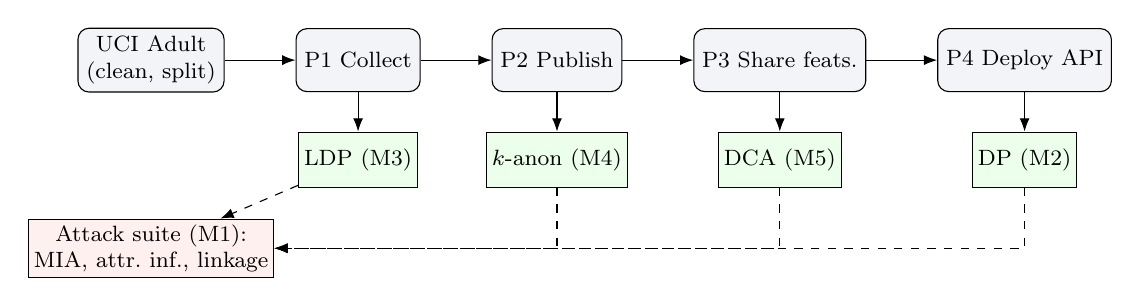
\begin{tikzpicture}[
  node distance=5mm and 9mm, >=Latex, font=\footnotesize,
  box/.style={draw, rounded corners, align=center, minimum height=8mm, fill=accent!6, inner sep=3pt},
  atk/.style={draw, align=center, minimum height=7mm, fill=red!6, inner sep=2pt},
  def/.style={draw, align=center, minimum height=7mm, fill=green!8, inner sep=2pt}]
\node[box] (data) {UCI Adult\\(clean, split)};
\node[box, right=of data] (p1) {P1 Collect};
\node[box, right=of p1] (p2) {P2 Publish};
\node[box, right=of p2] (p3) {P3 Share feats.};
\node[box, right=of p3] (p4) {P4 Deploy API};
\draw[->] (data)--(p1); \draw[->] (p1)--(p2); \draw[->] (p2)--(p3); \draw[->] (p3)--(p4);
\node[def, below=of p1] (d1) {LDP (M3)};
\node[def, below=of p2] (d2) {$k$-anon (M4)};
\node[def, below=of p3] (d3) {DCA (M5)};
\node[def, below=of p4] (d4) {DP (M2)};
\draw[->] (p1)--(d1); \draw[->] (p2)--(d2); \draw[->] (p3)--(d3); \draw[->] (p4)--(d4);
\node[atk, below=16mm of data] (atk) {Attack suite (M1):\\ MIA, attr.\ inf., linkage};
\draw[->, dashed] (d1)--(atk); \draw[->, dashed] (d2)|-(atk);
\draw[->, dashed] (d3)|-(atk); \draw[->, dashed] (d4)|-(atk);
\end{tikzpicture}
\caption{Common evaluation pipeline. Each exposure point $P_i$ receives the module
mechanism matched to it; the Module-1 attack suite scores utility and privacy on
identical data splits.}\label{fig:flow}
\end{figure}

% ================================================================== 3
\section{Dataset Identification and Preliminary Preparation}\label{sec:data}
\textbf{Source and licence.} UCI \emph{Adult} / Census Income
\citep{adultuci} (Becker \& Kohavi, 1996; DOI 10.24432/C5XW20), released under
CC~BY~4.0 -- lawfully usable with attribution.

\noindent\textbf{Suitability.} It is the canonical privacy-ML benchmark: it carries
real quasi-identifiers (age, sex, race, marital status, education, native country)
and a natural sensitive attribute (sex), so every module's mechanism has a genuine
target. Its known limitation -- it is a stale 1994 extract with demographic skew
\citep{ding2021retiring} -- motivates the IA-2 replication on ACSIncome.

\noindent\textbf{Preparation log.} Whitespace stripped; \texttt{?} mapped to missing;
rows with any missing value dropped; income mapped to $\{0,1\}$; the survey weight
\texttt{fnlwgt} excluded; categoricals one-hot encoded and numerics standardised on
\emph{training} statistics only. This yields \NTrain{} training and \NTest{} test
records ($\NFeat$ encoded features; positive rate \PosRate), from 48{,}842 raw rows.
Cleaned splits and SHA-256 hashes are recorded in \texttt{data/PROVENANCE.md} and
\texttt{data/processed/processed\_manifest.json}.

% ================================================================== 4
\section{Initial Implementation and Demonstration}\label{sec:impl}
All code is in \texttt{src/privpipe/} (mechanisms written from scratch; Opacus used
only for the DP-SGD accountant) and is exercised by \texttt{IA1/scripts\_ia1.py};
mechanism correctness is checked in \texttt{tests/} (13 passing tests).

\subsection{Utility baselines and the deployment-layer attack}
Table~\ref{tab:baselines} reports four classifiers and a loss-threshold membership
inference attack (MIA) on each. \BestModel{} is the strongest classifier
(\BestAcc{} accuracy). The Random Forest, which overfits, is the most leak-prone:
its MIA AUC is \RFMIA{} (advantage \RFAdv{}), empirically linking privacy risk to
overfitting \citep{yeom2018privacy}.
\begin{table}[htbp]\centering\caption{Utility baselines and loss-threshold MIA (mean over 3 seeds).}\label{tab:baselines}
\begin{tabular}{lrrrrr}
\toprule
Model & Acc. & $F_1$ & ROC-AUC & MIA AUC & MIA adv. \\
\midrule
Logistic Regression & 0.848 & 0.667 & 0.907 & 0.497 & -0.010 \\
Gaussian Naive Bayes & 0.644 & 0.563 & 0.854 & 0.498 & -0.002 \\
Random Forest & 0.842 & 0.666 & 0.892 & 0.592 & 0.108 \\
MLP & 0.828 & 0.634 & 0.875 & 0.532 & 0.017 \\
\bottomrule
\end{tabular}

\end{table}

\subsection{The ``just drop the sensitive column'' fallacy}
Removing \texttt{sex} does not hide it: an adversary reconstructs it from the
remaining attributes with accuracy \AIacc{} versus a majority baseline of \AIbase{}
(a leakage of \AIleak{}). This is the demonstration that motivates genuine
mechanisms rather than naive suppression.

\subsection{Publishing-layer linkage risk}
Table~\ref{tab:qi} shows that \FracUnique{} of records are \emph{unique} on their
quasi-identifiers (achieved $k=1$), i.e.\ directly re-identifiable -- the risk that
$k$-anonymity must remove.
\begin{table}[htbp]\centering\caption{Quasi-identifier uniqueness / linkage risk.}\label{tab:qi}
\begin{tabular}{lrrrr}
\toprule
Age bin & Frac. unique & Frac.\ $\le2$ & Achieved $k$ & \#classes \\
\midrule
1 & 0.138 & 0.191 & 1 & 9880 \\
5 & 0.073 & 0.105 & 1 & 5441 \\
10 & 0.055 & 0.080 & 1 & 4196 \\
\bottomrule
\end{tabular}

\end{table}

\subsection{Module 2 --- DP Naive Bayes}
Table~\ref{tab:dpnb} and Figure~\ref{fig:dpnb} give a first $\varepsilon$ sweep for a
scratch DP Naive Bayes (Laplace noise on class-conditional counts). Utility is
near-flat across $\varepsilon\in[0.5,5]$, indicating the binned-count mechanism is
noise-tolerant on this dataset -- a first data point for the trade-off curves.
\begin{minipage}{0.52\textwidth}\centering\captionof{table}{DP Naive Bayes $\varepsilon$ sweep.}\label{tab:dpnb}
\begin{tabular}{lrrrr}
\toprule
$\varepsilon$ & Acc. & Bal. Acc. & $F_1$ & ROC-AUC \\
\midrule
0.5 & 0.767 & 0.755 & 0.609 & 0.835 \\
1.0 & 0.756 & 0.757 & 0.607 & 0.855 \\
2.0 & 0.754 & 0.758 & 0.607 & 0.859 \\
5.0 & 0.753 & 0.760 & 0.608 & 0.860 \\
$\infty$ & 0.644 & 0.738 & 0.563 & 0.854 \\
\bottomrule
\end{tabular}
\end{minipage}\hfill
\begin{minipage}{0.45\textwidth}\centering
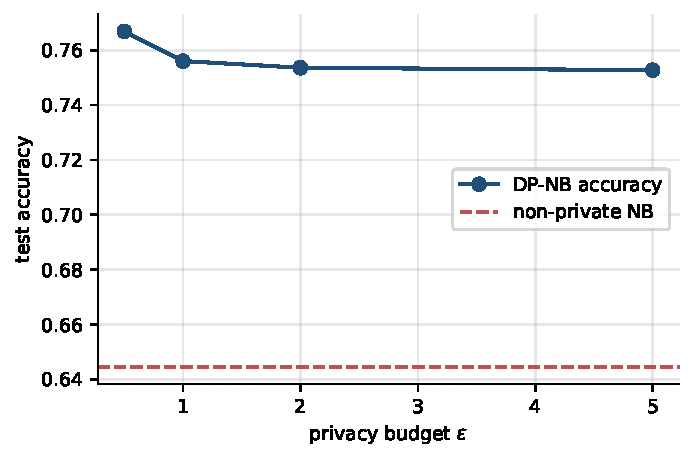
\includegraphics[width=\linewidth]{figs/dpnb_sweep.pdf}
\captionof{figure}{DP-NB accuracy vs $\varepsilon$.}\label{fig:dpnb}
\end{minipage}

\subsection{Module 3 --- LDP frequency oracles}
Figure~\ref{fig:ldp} and Table~\ref{tab:ldp} estimate the \texttt{education}
distribution under GRR and OUE. OUE's mean-squared error is one to two orders of
magnitude below GRR's at small $\varepsilon$, matching the theory that unary
encoding dominates generalised randomised response on larger domains
\citep{wang2017locally}.
\begin{minipage}{0.45\textwidth}\centering
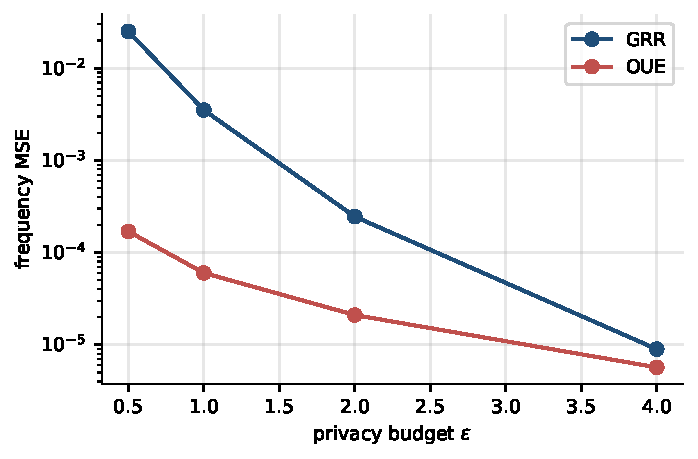
\includegraphics[width=\linewidth]{figs/ldp_mse.pdf}
\captionof{figure}{LDP frequency MSE vs $\varepsilon$ (log scale).}\label{fig:ldp}
\end{minipage}\hfill
\begin{minipage}{0.52\textwidth}\centering\captionof{table}{LDP frequency-estimation MSE on \texttt{education}.}\label{tab:ldp}
\begin{tabular}{lrr}
\toprule
$\varepsilon$ & GRR MSE & OUE MSE \\
\midrule
0.5 & 2.51e-02 & 1.70e-04 \\
1.0 & 3.52e-03 & 6.01e-05 \\
2.0 & 2.45e-04 & 2.10e-05 \\
4.0 & 8.96e-06 & 5.68e-06 \\
\bottomrule
\end{tabular}
\end{minipage}

\subsection{Module 4 --- Mondrian $k$-anonymity}
A scratch Mondrian anonymiser reaches the target $k=5$ exactly
(Table~\ref{tab:anon}), but exposes the classic weakness: five equivalence classes
are \emph{homogeneous} in the sensitive attribute (min $\ell=1$) and the worst-class
$t$-closeness is high. This is precisely the gap that $\ell$-diversity and
$t$-closeness close in IA-2.
\begin{table}[htbp]\centering\caption{Preliminary Mondrian $k$-anonymity ($k=5$) and its homogeneity weakness.}\label{tab:anon}
\begin{tabular}{lr}
\toprule
Property & Value \\
\midrule
Target $k$ & 5 \\
Achieved $k$ (min class size) & 5 \\
\#equivalence classes & 1123 \\
Min $\ell$ (distinct-$\ell$ diversity) & 1 \\
Homogeneous classes & 5 \\
Records disclosed by homogeneity & 0.001 \\
Worst-class $t$ (total-variation) & 0.889 \\
\bottomrule
\end{tabular}

\end{table}

\subsection{Module 5 --- compressive privacy}
Table~\ref{tab:comp} compresses the 103-dimensional features to $p=10$ and reports
both utility (income accuracy) and leakage (how well the sensitive \texttt{sex}
label survives). PCA preserves \emph{everything}, so sex is recovered at accuracy
\PCAsex{}; privacy-aware DCA keeps income accuracy high (\PADCAincome{}) while
cutting sex recovery to \PADCAsex{} -- the compressive-privacy trade-off in a single
row.
\begin{table}[htbp]\centering\caption{Preliminary PCA vs DCA ($p=10$): utility is income accuracy, leakage is sex accuracy.}\label{tab:comp}
\begin{tabular}{lrrr}
\toprule
Projection ($p{=}10$) & Income acc.\ (utility) & Sex acc.\ (leakage) & Recon.\ err. \\
\midrule
PCA & 0.839 & 1.000 & 0.492 \\
DCA & 0.844 & 0.831 & 0.751 \\
pa-DCA & 0.840 & 0.689 & 0.780 \\
random & 0.790 & 0.913 & 0.688 \\
\bottomrule
\end{tabular}

\end{table}

% ================================================================== 5
\section{Preliminary Evaluation and Documentation}\label{sec:eval}

\subsection{Observations}
\begin{itemize}
\item Overfitting drives leakage: the RF's high MIA AUC (\RFMIA{}) confirms the
overfitting--privacy link and justifies DP at the deployment layer.
\item Suppression fails (attribute leakage \AIleak{} above baseline); real
mechanisms are needed.
\item Each module's preliminary mechanism already shows its signature trade-off:
OUE $\gg$ GRR in accuracy; DP-NB noise-tolerant; Mondrian attains $k$ but not
$\ell$; privacy-aware DCA suppresses the sensitive label at little utility cost.
\end{itemize}

\subsection{Evaluation measures (for IA-2)}
Utility: accuracy, balanced accuracy, $F_1$, ROC-AUC. Privacy: $\varepsilon$
(at $\delta=10^{-5}$), $k/\ell/t$; MIA AUC, advantage and TPR@1\%FPR
\citep{carlini2022membership}; attribute-inference accuracy over baseline;
re-identification rate; LDP estimator MSE vs theory. All IA-2 results will be
averaged over 5 seeds with mean\,$\pm$\,std.

\subsection{Known limitations and remaining work}
Single dataset and a US-centric 1994 vintage (addressed by the ACSIncome
replication); preliminary mechanisms use fixed hyper-parameters (IA-2 adds full
$\varepsilon$ sweeps and shadow-model MIA); the coverage matrix and the layered
DCA\,$+$\,DP-SGD combination are the main IA-2 deliverables.

\subsection{Individual-contribution statement}
\begin{shaded}\small
\noindent I, \textbf{Deon Ajit Menezes} (16014223030, B1), independently designed the
four-exposure framing and the single-benchmark methodology, and wrote the
\texttt{privpipe} package from scratch -- the data pipeline, the membership /
attribute / linkage attacks, the DP Naive Bayes, the LDP frequency and numeric
oracles, the Mondrian anonymiser with the $\ell$-diversity and $t$-closeness
checks, and the PCA/DCA compressive-privacy module -- together with the unit tests
and the experiment driver that produced every number above. Opacus is used only as
the DP-SGD privacy accountant in IA-2; all other mechanisms are my own
implementation.
\end{shaded}

\bibliographystyle{plainnat}
\bibliography{refs}
\end{document}
